In-context function estimation is the task of estimating the underlying function given a set of context points that have been sampled from that function or an empirical process. Using the estimated function, it is possible to impute missing data points. \cite{seifner2025zeroshotimputationfoundationinference}

This can be done using an underlying model assumption like with linear regression. A polynomial of a certain order is fitted to the given data, determining which parameters fit best to the data. For linear regression, it is assumed that the underlying function can be modeled by a polynomial. The order of this polynomial must be determined in advance. Due to the best-fit approach, linear regression is not able to handle uncertainties that might result from missing data.

Gaussian Processes (GP) are a way of estimating missing values that takes uncertainties into account. GPs assume a prior distribution of possible underlying functions and update that belief based on the given context points. This has to be done individually for each data frame. \cite{garnelo2018neural}

\autoref{fig:gaussian} shows some results of fitting Gaussian Processes on given context points while knowing the prior distribution from which the true underlying function has been sampled. This posterior distribution defines a mean and standard deviation value for each point in the grid. In the leftmost plot, it is visible that missing data from about $x=0.6$ to $x=1$ leads to high uncertainty. The rightmost plot shows uncertainty spikes between context points. This is due to the low RBF-Score. Sampling with a low RBF Score results in strongly varying functions. Therefore, the GP assumes that the function value can vary a lot, resulting in uncertainty spikes even between context points that are comparatively close on the x-axis. TODO: verify this statement 

\begin{figure*}
	\centering
	\resizebox{0.90\textwidth}{!}{
		% This file was created with matplot2tikz v0.4.0.
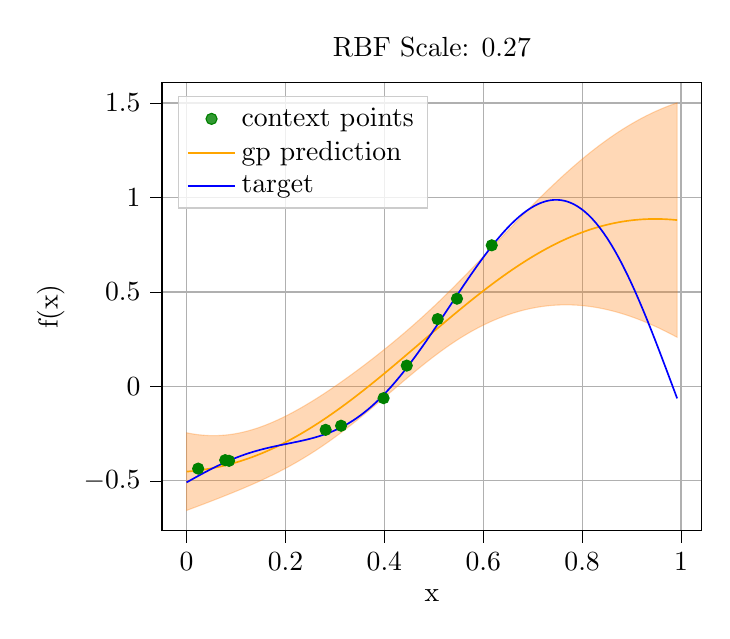
\begin{tikzpicture}

\definecolor{darkgray176}{RGB}{176,176,176}
\definecolor{darkorange25512714}{RGB}{255,127,14}
\definecolor{green}{RGB}{0,128,0}
\definecolor{lightgray204}{RGB}{204,204,204}
\definecolor{orange}{RGB}{255,165,0}

\begin{axis}[
legend cell align={left},
legend style={
  fill opacity=0.8,
  draw opacity=1,
  text opacity=1,
  at={(0.03,0.97)},
  anchor=north west,
  draw=lightgray204
},
tick align=outside,
tick pos=left,
title={RBF Scale: 0.27},
x grid style={darkgray176},
xlabel={x},
xmajorgrids,
xmin=-0.049609375, xmax=1.041796875,
xtick style={color=black},
y grid style={darkgray176},
ylabel={f(x)},
ymajorgrids,
ymin=-0.764390990198043, ymax=1.60873415540691,
ytick style={color=black}
]
\path [draw=darkorange25512714, fill=darkorange25512714, opacity=0.3]
(axis cs:0,-0.245463616773546)
--(axis cs:0,-0.656521665397818)
--(axis cs:0.0078125,-0.648969787345521)
--(axis cs:0.015625,-0.641357306466875)
--(axis cs:0.0234375,-0.63368574994382)
--(axis cs:0.03125,-0.625956021297951)
--(axis cs:0.0390625,-0.618168265902341)
--(axis cs:0.046875,-0.610321734795528)
--(axis cs:0.0546875,-0.602414652145809)
--(axis cs:0.0625,-0.594444092638462)
--(axis cs:0.0703125,-0.586405875687576)
--(axis cs:0.078125,-0.578294483568065)
--(axis cs:0.0859375,-0.570103010207164)
--(axis cs:0.09375,-0.561823146403661)
--(axis cs:0.1015625,-0.553445205666003)
--(axis cs:0.109375,-0.54495819277212)
--(axis cs:0.1171875,-0.536349914731901)
--(axis cs:0.125,-0.527607131317794)
--(axis cs:0.1328125,-0.518715739986708)
--(axis cs:0.140625,-0.509660988097148)
--(axis cs:0.1484375,-0.500427704021322)
--(axis cs:0.15625,-0.491000538167458)
--(axis cs:0.1640625,-0.481364205068657)
--(axis cs:0.171875,-0.471503718477013)
--(axis cs:0.1796875,-0.461404612673858)
--(axis cs:0.1875,-0.451053144782813)
--(axis cs:0.1953125,-0.440436474562818)
--(axis cs:0.203125,-0.42954281979833)
--(axis cs:0.2109375,-0.418361586868234)
--(axis cs:0.21875,-0.406883477285022)
--(axis cs:0.2265625,-0.395100571916639)
--(axis cs:0.234375,-0.383006395236394)
--(axis cs:0.2421875,-0.370595962318183)
--(axis cs:0.25,-0.357865811446516)
--(axis cs:0.2578125,-0.344814025190627)
--(axis cs:0.265625,-0.331440242645226)
--(axis cs:0.2734375,-0.317745665308054)
--(axis cs:0.28125,-0.303733058778389)
--(axis cs:0.2890625,-0.289406752145637)
--(axis cs:0.296875,-0.274772636608218)
--(axis cs:0.3046875,-0.259838164528601)
--(axis cs:0.3125,-0.244612349792445)
--(axis cs:0.3203125,-0.229105769995019)
--(axis cs:0.328125,-0.213330570619701)
--(axis cs:0.3359375,-0.197300470991879)
--(axis cs:0.34375,-0.181030771376391)
--(axis cs:0.3515625,-0.16453836012762)
--(axis cs:0.359375,-0.147841719290765)
--(axis cs:0.3671875,-0.130960926487913)
--(axis cs:0.375,-0.113917650308875)
--(axis cs:0.3828125,-0.0967351357823525)
--(axis cs:0.390625,-0.0794381758625024)
--(axis cs:0.3984375,-0.0620530642859241)
--(axis cs:0.40625,-0.044607524715748)
--(axis cs:0.4140625,-0.0271306109000974)
--(axis cs:0.421875,-0.00965257276066872)
--(axis cs:0.4296875,0.00779531596769478)
--(axis cs:0.4375,0.025180971576287)
--(axis cs:0.4453125,0.0424717566524391)
--(axis cs:0.453125,0.0596347769224114)
--(axis cs:0.4609375,0.0766372133872483)
--(axis cs:0.46875,0.0934466807042754)
--(axis cs:0.4765625,0.110031599072629)
--(axis cs:0.484375,0.126361563791065)
--(axis cs:0.4921875,0.142407694730738)
--(axis cs:0.5,0.158142947678924)
--(axis cs:0.5078125,0.173542371124558)
--(axis cs:0.515625,0.188583295530508)
--(axis cs:0.5234375,0.203245447095345)
--(axis cs:0.53125,0.217510983796849)
--(axis cs:0.5390625,0.231364457334044)
--(axis cs:0.546875,0.244792709670818)
--(axis cs:0.5546875,0.257784716639041)
--(axis cs:0.5625,0.27033139316796)
--(axis cs:0.5703125,0.282425375155786)
--(axis cs:0.578125,0.294060792025957)
--(axis cs:0.5859375,0.305233042008866)
--(axis cs:0.59375,0.315938579606615)
--(axis cs:0.6015625,0.32617472194545)
--(axis cs:0.609375,0.335939478119472)
--(axis cs:0.6171875,0.345231403389611)
--(axis cs:0.625,0.354049478327175)
--(axis cs:0.6328125,0.362393011699704)
--(axis cs:0.640625,0.370261565049039)
--(axis cs:0.6484375,0.377654896435808)
--(axis cs:0.65625,0.384572920637968)
--(axis cs:0.6640625,0.391015683112776)
--(axis cs:0.671875,0.396983345191297)
--(axis cs:0.6796875,0.40247617821551)
--(axis cs:0.6875,0.407494564607628)
--(axis cs:0.6953125,0.412039004149414)
--(axis cs:0.703125,0.416110124026287)
--(axis cs:0.7109375,0.419708691445336)
--(axis cs:0.71875,0.422835627861973)
--(axis cs:0.7265625,0.425492024045201)
--(axis cs:0.734375,0.427679155376855)
--(axis cs:0.7421875,0.429398496917998)
--(axis cs:0.75,0.430651737888901)
--(axis cs:0.7578125,0.43144079530088)
--(axis cs:0.765625,0.431767826552003)
--(axis cs:0.7734375,0.431635240857178)
--(axis cs:0.78125,0.431045709429203)
--(axis cs:0.7890625,0.430002174363149)
--(axis cs:0.796875,0.428507856204094)
--(axis cs:0.8046875,0.42656626019924)
--(axis cs:0.8125,0.424181181251318)
--(axis cs:0.8203125,0.42135670760188)
--(axis cs:0.828125,0.418097223281669)
--(axis cs:0.8359375,0.414407409371304)
--(axis cs:0.84375,0.410292244119685)
--(axis cs:0.8515625,0.405757001970285)
--(axis cs:0.859375,0.400807251547073)
--(axis cs:0.8671875,0.395448852652699)
--(axis cs:0.875,0.389687952331723)
--(axis cs:0.8828125,0.383530980051518)
--(axis cs:0.890625,0.376984642052911)
--(axis cs:0.8984375,0.370055914921896)
--(axis cs:0.90625,0.362752038432877)
--(axis cs:0.9140625,0.355080507712899)
--(axis cs:0.921875,0.34704906477532)
--(axis cs:0.9296875,0.338665689470253)
--(axis cs:0.9375,0.329938589898115)
--(axis cs:0.9453125,0.320876192331425)
--(axis cs:0.953125,0.311487130689041)
--(axis cs:0.9609375,0.301780235605857)
--(axis cs:0.96875,0.29176452313998)
--(axis cs:0.9765625,0.281449183158375)
--(axis cs:0.984375,0.270843567440861)
--(axis cs:0.9921875,0.259957177541405)
--(axis cs:0.9921875,1.50086483060668)
--(axis cs:0.9921875,1.50086483060668)
--(axis cs:0.984375,1.49378672161481)
--(axis cs:0.9765625,1.48627828092629)
--(axis cs:0.96875,1.47833775498946)
--(axis cs:0.9609375,1.46996378923872)
--(axis cs:0.953125,1.4611554366848)
--(axis cs:0.9453125,1.45191216620298)
--(axis cs:0.9375,1.44223387051589)
--(axis cs:0.9296875,1.43212087386868)
--(axis cs:0.921875,1.42157393939636)
--(axis cs:0.9140625,1.41059427618457)
--(axis cs:0.90625,1.39918354602732)
--(axis cs:0.8984375,1.38734386988692)
--(axis cs:0.890625,1.37507783406349)
--(axis cs:0.8828125,1.36238849608386)
--(axis cs:0.875,1.34927939032175)
--(axis cs:0.8671875,1.33575453336357)
--(axis cs:0.859375,1.32181842913672)
--(axis cs:0.8515625,1.30747607381963)
--(axis cs:0.84375,1.29273296055538)
--(axis cs:0.8359375,1.27759508399304)
--(axis cs:0.828125,1.26206894468325)
--(axis cs:0.8203125,1.24616155335654)
--(axis cs:0.8125,1.22988043511461)
--(axis cs:0.8046875,1.21323363356595)
--(axis cs:0.796875,1.1962297149376)
--(axis cs:0.7890625,1.17887777219414)
--(axis cs:0.78125,1.16118742919319)
--(axis cs:0.7734375,1.14316884490261)
--(axis cs:0.765625,1.12483271769844)
--(axis cs:0.7578125,1.10619028975321)
--(axis cs:0.75,1.08725335151067)
--(axis cs:0.7421875,1.06803424622434)
--(axis cs:0.734375,1.04854587451213)
--(axis cs:0.7265625,1.02880169884586)
--(axis cs:0.71875,1.00881574785079)
--(axis cs:0.7109375,0.988602620234382)
--(axis cs:0.703125,0.968177488092129)
--(axis cs:0.6953125,0.947556099248853)
--(axis cs:0.6875,0.926754778183207)
--(axis cs:0.6796875,0.905790424947568)
--(axis cs:0.671875,0.884680511332584)
--(axis cs:0.6640625,0.863443073332829)
--(axis cs:0.65625,0.84209669874664)
--(axis cs:0.6484375,0.820660508491282)
--(axis cs:0.640625,0.799154129939792)
--(axis cs:0.6328125,0.7775976602999)
--(axis cs:0.625,0.756011617778037)
--(axis cs:0.6171875,0.734416878032577)
--(axis cs:0.609375,0.712834593262721)
--(axis cs:0.6015625,0.691286091259701)
--(axis cs:0.59375,0.669792751935384)
--(axis cs:0.5859375,0.648375859320834)
--(axis cs:0.578125,0.627056427876995)
--(axis cs:0.5703125,0.605855003252754)
--(axis cs:0.5625,0.584791439401924)
--(axis cs:0.5546875,0.563884656211629)
--(axis cs:0.546875,0.543152384397029)
--(axis cs:0.5390625,0.52261090717137)
--(axis cs:0.53125,0.502274810784686)
--(axis cs:0.5234375,0.48215675802718)
--(axis cs:0.515625,0.462267299767571)
--(axis cs:0.5078125,0.442614739148324)
--(axis cs:0.5,0.423205060951432)
--(axis cs:0.4921875,0.404041934894077)
--(axis cs:0.484375,0.38512679652759)
--(axis cs:0.4765625,0.366459003588864)
--(axis cs:0.46875,0.348036059863965)
--(axis cs:0.4609375,0.329853893665936)
--(axis cs:0.453125,0.311907174554528)
--(axis cs:0.4453125,0.294189650310489)
--(axis cs:0.4375,0.27669448646339)
--(axis cs:0.4296875,0.259414592597007)
--(axis cs:0.421875,0.242342922745781)
--(axis cs:0.4140625,0.225472740889473)
--(axis cs:0.40625,0.208797846319522)
--(axis cs:0.3984375,0.192312757072031)
--(axis cs:0.390625,0.176012852430631)
--(axis cs:0.3828125,0.159894477579337)
--(axis cs:0.375,0.143955014833442)
--(axis cs:0.3671875,0.12819292658027)
--(axis cs:0.359375,0.112607775248498)
--(axis cs:0.3515625,0.0972002254337523)
--(axis cs:0.34375,0.0819720328681524)
--(axis cs:0.3359375,0.0669260243395844)
--(axis cs:0.328125,0.0520660720241412)
--(axis cs:0.3203125,0.037397065048796)
--(axis cs:0.3125,0.022924880485652)
--(axis cs:0.3046875,0.0086563554121587)
--(axis cs:0.296875,-0.0054007388411354)
--(axis cs:0.2890625,-0.0192377195949132)
--(axis cs:0.28125,-0.0328450126346484)
--(axis cs:0.2734375,-0.0462121690742715)
--(axis cs:0.265625,-0.0593278797716453)
--(axis cs:0.2578125,-0.0721799881446169)
--(axis cs:0.25,-0.0847555025768614)
--(axis cs:0.2421875,-0.0970406099394468)
--(axis cs:0.234375,-0.109020692085459)
--(axis cs:0.2265625,-0.120680347492559)
--(axis cs:0.21875,-0.13200342051674)
--(axis cs:0.2109375,-0.14297304095551)
--(axis cs:0.203125,-0.153571676767881)
--(axis cs:0.1953125,-0.163781202821176)
--(axis cs:0.1875,-0.173582988384893)
--(axis cs:0.1796875,-0.182958005722401)
--(axis cs:0.171875,-0.191886961500601)
--(axis cs:0.1640625,-0.2003504518192)
--(axis cs:0.15625,-0.208329140453493)
--(axis cs:0.1484375,-0.215803958442461)
--(axis cs:0.140625,-0.22275632151615)
--(axis cs:0.1328125,-0.229168360167916)
--(axis cs:0.125,-0.235023155603417)
--(axis cs:0.1171875,-0.240304973528026)
--(axis cs:0.109375,-0.244999486953931)
--(axis cs:0.1015625,-0.249093979068916)
--(axis cs:0.09375,-0.25257751779508)
--(axis cs:0.0859375,-0.25544109497167)
--(axis cs:0.078125,-0.257677725017003)
--(axis cs:0.0703125,-0.259282500268301)
--(axis cs:0.0625,-0.260252602715121)
--(axis cs:0.0546875,-0.260587274265309)
--(axis cs:0.046875,-0.260287749771927)
--(axis cs:0.0390625,-0.259357158627849)
--(axis cs:0.03125,-0.257800401706798)
--(axis cs:0.0234375,-0.255624010786819)
--(axis cs:0.015625,-0.252835997399073)
--(axis cs:0.0078125,-0.249445697416571)
--(axis cs:0,-0.245463616773546)
--cycle;

\addplot [draw=green, fill=green, mark=*, only marks]
table{%
x  y
0.0234375 -0.435152769088745
0.078125 -0.390416473150253
0.0859375 -0.39392226934433
0.28125 -0.229927331209183
0.3125 -0.208194002509117
0.3984375 -0.0621931217610836
0.4453125 0.110128581523895
0.5078125 0.356279462575912
0.546875 0.46435934305191
0.6171875 0.746831953525543
};
\addlegendentry{context points}
\addplot [semithick, orange]
table {%
0 -0.450992641085682
0.0078125 -0.449207742381046
0.015625 -0.447096651932974
0.0234375 -0.444654880365319
0.03125 -0.441878211502374
0.0390625 -0.438762712265095
0.046875 -0.435304742283728
0.0546875 -0.431500963205559
0.0625 -0.427348347676792
0.0703125 -0.422844187977939
0.078125 -0.417986104292534
0.0859375 -0.412772052589417
0.09375 -0.40720033209937
0.1015625 -0.401269592367459
0.109375 -0.394978839863025
0.1171875 -0.388327444129963
0.125 -0.381315143460606
0.1328125 -0.373942050077312
0.140625 -0.366208654806649
0.1484375 -0.358115831231892
0.15625 -0.349664839310475
0.1640625 -0.340857328443928
0.171875 -0.331695339988807
0.1796875 -0.322181309198129
0.1875 -0.312318066583853
0.1953125 -0.302108838691997
0.203125 -0.291557248283106
0.2109375 -0.280667313911872
0.21875 -0.269443448900881
0.2265625 -0.257890459704599
0.234375 -0.246013543660927
0.2421875 -0.233818286128815
0.25 -0.221310657011689
0.2578125 -0.208497006667622
0.265625 -0.195384061208436
0.2734375 -0.181978917191163
0.28125 -0.168289035706519
0.2890625 -0.154322235870275
0.296875 -0.140086687724677
0.3046875 -0.125590904558221
0.3125 -0.110843734653396
0.3203125 -0.0958543524731112
0.328125 -0.0806322492977798
0.3359375 -0.0651872233261472
0.34375 -0.0495293692541194
0.3515625 -0.033669067346934
0.359375 -0.0176169720211337
0.3671875 -0.00138399995382166
0.375 0.0150186822622835
0.3828125 0.0315796708984921
0.390625 0.0482873382840641
0.3984375 0.0651298463930532
0.40625 0.0820951608018872
0.4140625 0.099171064994688
0.421875 0.116345174992556
0.4296875 0.133604954282351
0.4375 0.150937729019839
0.4453125 0.168330703481464
0.453125 0.18577097573847
0.4609375 0.203245553526592
0.46875 0.22074137028412
0.4765625 0.238245301330746
0.484375 0.255744180159328
0.4921875 0.273224814812407
0.5 0.290674004315178
0.5078125 0.308078555136441
0.515625 0.32542529764904
0.5234375 0.342701102561263
0.53125 0.359892897290767
0.5390625 0.376987682252707
0.546875 0.393972547033924
0.5546875 0.410834686425335
0.5625 0.427561416284942
0.5703125 0.44414018920427
0.578125 0.460558609951476
0.5859375 0.47680445066485
0.59375 0.492865665770999
0.6015625 0.508730406602576
0.609375 0.524387035691096
0.6171875 0.539824140711094
0.625 0.555030548052606
0.6328125 0.569995335999802
0.640625 0.584707847494415
0.6484375 0.599157702463545
0.65625 0.613334809692304
0.6640625 0.627229378222802
0.671875 0.64083192826194
0.6796875 0.654133301581539
0.6875 0.667124671395418
0.6953125 0.679797551699133
0.703125 0.692143806059208
0.7109375 0.704155655839859
0.71875 0.71582568785638
0.7265625 0.727146861445529
0.734375 0.738112514944491
0.7421875 0.748716371571168
0.75 0.758952544699787
0.7578125 0.768815542527047
0.765625 0.778300272125222
0.7734375 0.787402042879894
0.78125 0.796116569311196
0.7890625 0.804439973278643
0.796875 0.812368785570846
0.8046875 0.819899946882597
0.8125 0.827030808182964
0.8203125 0.83375913047921
0.828125 0.840083083982458
0.8359375 0.84600124668217
0.84375 0.851512602337531
0.8515625 0.856616537894956
0.859375 0.861312840341896
0.8671875 0.865601693008134
0.875 0.869483671326735
0.8828125 0.872959738067687
0.890625 0.876031238058199
0.8984375 0.878699892404409
0.90625 0.880967792230101
0.9140625 0.882837391948734
0.921875 0.884311502085841
0.9296875 0.885393281669469
0.9375 0.886086230207001
0.9453125 0.886394179267202
0.953125 0.886321283686921
0.9609375 0.885872012422291
0.96875 0.885051139064719
0.9765625 0.883863732042332
0.984375 0.882315144527836
0.9921875 0.880411004074045
};
\addlegendentry{gp prediction}
\addplot [semithick, blue]
table {%
0 -0.50814962387085
0.0078125 -0.496681034564972
0.015625 -0.485288977622986
0.0234375 -0.474015474319458
0.03125 -0.46290135383606
0.0390625 -0.451987385749817
0.046875 -0.441312849521637
0.0546875 -0.430915027856827
0.0625 -0.420828431844711
0.0703125 -0.411084443330765
0.078125 -0.401710242033005
0.0859375 -0.392728626728058
0.09375 -0.384157747030258
0.1015625 -0.376009970903397
0.109375 -0.368293344974518
0.1171875 -0.361008644104004
0.125 -0.354151487350464
0.1328125 -0.347710967063904
0.140625 -0.341671019792557
0.1484375 -0.336008131504059
0.15625 -0.330694168806076
0.1640625 -0.32569432258606
0.171875 -0.32096928358078
0.1796875 -0.316473960876465
0.1875 -0.312158674001694
0.1953125 -0.3079694211483
0.203125 -0.303848713636398
0.2109375 -0.299735546112061
0.21875 -0.29556605219841
0.2265625 -0.291274398565292
0.234375 -0.286793500185013
0.2421875 -0.282055079936981
0.25 -0.27699014544487
0.2578125 -0.271531194448471
0.265625 -0.265610426664352
0.2734375 -0.259162724018097
0.28125 -0.252124667167664
0.2890625 -0.244435146450996
0.296875 -0.236037015914917
0.3046875 -0.226876229047775
0.3125 -0.216903626918793
0.3203125 -0.206074655056
0.328125 -0.194348722696304
0.3359375 -0.18169204890728
0.34375 -0.168075278401375
0.3515625 -0.153475224971771
0.359375 -0.137874752283096
0.3671875 -0.121262766420841
0.375 -0.103634275496006
0.3828125 -0.084990382194519
0.390625 -0.0653383731842041
0.3984375 -0.0446914620697498
0.40625 -0.0230690203607082
0.4140625 -0.000495294865686446
0.421875 0.0229989755898714
0.4296875 0.0473779588937759
0.4375 0.0726012885570526
0.4453125 0.0986236706376076
0.453125 0.125395134091377
0.4609375 0.152861669659615
0.46875 0.180965840816498
0.4765625 0.209646478295326
0.484375 0.238839074969292
0.4921875 0.268476754426956
0.5 0.298489660024643
0.5078125 0.328806608915329
0.515625 0.359353482723236
0.5234375 0.390055239200592
0.53125 0.420835047960281
0.5390625 0.451615005731583
0.546875 0.482316374778748
0.5546875 0.512859582901001
0.5625 0.543164312839508
0.5703125 0.573149740695953
0.578125 0.602734863758087
0.5859375 0.631838083267212
0.59375 0.660378038883209
0.6015625 0.688272356987
0.609375 0.715439200401306
0.6171875 0.741796851158142
0.625 0.767262697219849
0.6328125 0.791754961013794
0.640625 0.815191507339478
0.6484375 0.837490320205688
0.65625 0.858569502830505
0.6640625 0.878347873687744
0.671875 0.8967444896698
0.6796875 0.913678407669067
0.6875 0.929070115089417
0.6953125 0.942841053009033
0.703125 0.954913258552551
0.7109375 0.965210914611816
0.71875 0.973659873008728
0.7265625 0.980187714099884
0.734375 0.984725594520569
0.7421875 0.987206816673279
0.75 0.987568557262421
0.7578125 0.98575222492218
0.765625 0.981703698635101
0.7734375 0.975374042987823
0.78125 0.966719806194305
0.7890625 0.95570433139801
0.796875 0.942297518253326
0.8046875 0.926477015018463
0.8125 0.908228397369385
0.8203125 0.887546002864838
0.828125 0.864433288574219
0.8359375 0.838903546333313
0.84375 0.810979902744293
0.8515625 0.780696392059326
0.859375 0.748097896575928
0.8671875 0.713239848613739
0.875 0.676189780235291
0.8828125 0.637026131153107
0.890625 0.595839262008667
0.8984375 0.552730083465576
0.90625 0.507811665534973
0.9140625 0.461207449436188
0.921875 0.413051575422287
0.9296875 0.363487958908081
0.9375 0.312670201063156
0.9453125 0.260761171579361
0.953125 0.207931026816368
0.9609375 0.154357388615608
0.96875 0.100224360823631
0.9765625 0.0457205921411514
0.984375 -0.00896052457392216
0.9921875 -0.0636230930685997
};
\addlegendentry{target}
\end{axis}

\end{tikzpicture}

		% This file was created with matplot2tikz v0.4.0.
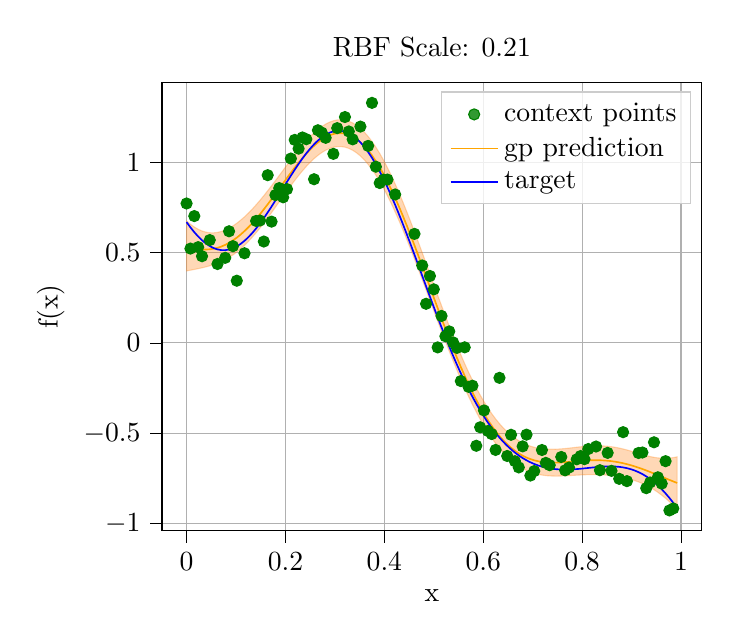
\begin{tikzpicture}

\definecolor{darkgray176}{RGB}{176,176,176}
\definecolor{darkorange25512714}{RGB}{255,127,14}
\definecolor{green}{RGB}{0,128,0}
\definecolor{lightgray204}{RGB}{204,204,204}
\definecolor{orange}{RGB}{255,165,0}

\begin{axis}[
legend cell align={left},
legend style={fill opacity=0.8, draw opacity=1, text opacity=1, draw=lightgray204},
tick align=outside,
tick pos=left,
title={RBF Scale: 0.21},
x grid style={darkgray176},
xlabel={x},
xmajorgrids,
xmin=-0.049609375, xmax=1.041796875,
xtick style={color=black},
y grid style={darkgray176},
ylabel={f(x)},
ymajorgrids,
ymin=-1.03975863456726, ymax=1.44098014831543,
ytick style={color=black}
]
\path [draw=darkorange25512714, fill=darkorange25512714, opacity=0.3]
(axis cs:0,0.674425466042734)
--(axis cs:0,0.398245043076177)
--(axis cs:0.0078125,0.402341016518767)
--(axis cs:0.015625,0.40650681290413)
--(axis cs:0.0234375,0.410860250838664)
--(axis cs:0.03125,0.41553690032933)
--(axis cs:0.0390625,0.420694940013351)
--(axis cs:0.046875,0.426516902954857)
--(axis cs:0.0546875,0.433206272460823)
--(axis cs:0.0625,0.44097827024004)
--(axis cs:0.0703125,0.450046224461232)
--(axis cs:0.078125,0.460606462529595)
--(axis cs:0.0859375,0.472824864506443)
--(axis cs:0.09375,0.486827145078188)
--(axis cs:0.1015625,0.50269344200463)
--(axis cs:0.109375,0.520456659983196)
--(axis cs:0.1171875,0.540103527205876)
--(axis cs:0.125,0.561577329673432)
--(axis cs:0.1328125,0.584781533612999)
--(axis cs:0.140625,0.60958379057995)
--(axis cs:0.1484375,0.635820048173759)
--(axis cs:0.15625,0.663298639347697)
--(axis cs:0.1640625,0.691804305842112)
--(axis cs:0.171875,0.721102145778423)
--(axis cs:0.1796875,0.750941479690183)
--(axis cs:0.1875,0.781059617008577)
--(axis cs:0.1953125,0.811185486769957)
--(axis cs:0.203125,0.841043080419918)
--(axis cs:0.2109375,0.870354647556082)
--(axis cs:0.21875,0.898843591330824)
--(axis cs:0.2265625,0.92623702961251)
--(axis cs:0.234375,0.952268017471635)
--(axis cs:0.2421875,0.976677459421266)
--(axis cs:0.25,0.999215768145248)
--(axis cs:0.2578125,1.01964434361417)
--(axis cs:0.265625,1.03773694936156)
--(axis cs:0.2734375,1.05328105214166)
--(axis cs:0.28125,1.06607917118175)
--(axis cs:0.2890625,1.07595025905362)
--(axis cs:0.296875,1.0827311126736)
--(axis cs:0.3046875,1.08627779345275)
--(axis cs:0.3125,1.08646702176053)
--(axis cs:0.3203125,1.08319750279313)
--(axis cs:0.328125,1.07639113792894)
--(axis cs:0.3359375,1.06599407661671)
--(axis cs:0.34375,1.05197756768382)
--(axis cs:0.3515625,1.03433857474875)
--(axis cs:0.359375,1.01310012746222)
--(axis cs:0.3671875,0.988311388057379)
--(axis cs:0.375,0.960047420754759)
--(axis cs:0.3828125,0.928408659609905)
--(axis cs:0.390625,0.893520078124689)
--(axis cs:0.3984375,0.85553007111431)
--(axis cs:0.40625,0.814609065724769)
--(axis cs:0.4140625,0.770947883980946)
--(axis cs:0.421875,0.724755883733201)
--(axis cs:0.4296875,0.676258908355562)
--(axis cs:0.4375,0.62569707809052)
--(axis cs:0.4453125,0.573322457645693)
--(axis cs:0.453125,0.519396635663933)
--(axis cs:0.4609375,0.464188252148346)
--(axis cs:0.46875,0.407970509939564)
--(axis cs:0.4765625,0.351018705971551)
--(axis cs:0.484375,0.293607817259691)
--(axis cs:0.4921875,0.236010175292232)
--(axis cs:0.5,0.178493260499594)
--(axis cs:0.5078125,0.12131764547365)
--(axis cs:0.515625,0.0647351112611923)
--(axis cs:0.5234375,0.0089869550522087)
--(axis cs:0.53125,-0.0456975002373638)
--(axis cs:0.5390625,-0.0991021934831955)
--(axis cs:0.546875,-0.151025419531493)
--(axis cs:0.5546875,-0.201280750090915)
--(axis cs:0.5625,-0.249697810172381)
--(axis cs:0.5703125,-0.29612294414358)
--(axis cs:0.578125,-0.340419805569217)
--(axis cs:0.5859375,-0.382469899231798)
--(axis cs:0.59375,-0.422173092579358)
--(axis cs:0.6015625,-0.459448099161465)
--(axis cs:0.609375,-0.494232921168605)
--(axis cs:0.6171875,-0.526485224941313)
--(axis cs:0.625,-0.556182614577307)
--(axis cs:0.6328125,-0.583322765623216)
--(axis cs:0.640625,-0.607923383025085)
--(axis cs:0.6484375,-0.630021953712427)
--(axis cs:0.65625,-0.649675272593312)
--(axis cs:0.6640625,-0.666958729596746)
--(axis cs:0.671875,-0.681965353425287)
--(axis cs:0.6796875,-0.694804614216893)
--(axis cs:0.6875,-0.705600992310477)
--(axis cs:0.6953125,-0.714492324193463)
--(axis cs:0.703125,-0.721627940210757)
--(axis cs:0.7109375,-0.727166612578513)
--(axis cs:0.71875,-0.731274337451322)
--(axis cs:0.7265625,-0.734121981765928)
--(axis cs:0.734375,-0.735882834419928)
--(axis cs:0.7421875,-0.736730111548268)
--(axis cs:0.75,-0.736834476092749)
--(axis cs:0.7578125,-0.736361640833116)
--(axis cs:0.765625,-0.735470129636292)
--(axis cs:0.7734375,-0.73430927221295)
--(axis cs:0.78125,-0.733017502294626)
--(axis cs:0.7890625,-0.731721018251978)
--(axis cs:0.796875,-0.730532850503909)
--(axis cs:0.8046875,-0.729552364388675)
--(axis cs:0.8125,-0.728865213634327)
--(axis cs:0.8203125,-0.72854375094701)
--(axis cs:0.828125,-0.728647900285244)
--(axis cs:0.8359375,-0.72922650046816)
--(axis cs:0.84375,-0.730319140657576)
--(axis cs:0.8515625,-0.731958521880248)
--(axis cs:0.859375,-0.73417338939159)
--(axis cs:0.8671875,-0.736992078183996)
--(axis cs:0.875,-0.740446680732619)
--(axis cs:0.8828125,-0.744577753367371)
--(axis cs:0.890625,-0.749439283928804)
--(axis cs:0.8984375,-0.755103303460491)
--(axis cs:0.90625,-0.76166302671204)
--(axis cs:0.9140625,-0.769232855360105)
--(axis cs:0.921875,-0.777943311100295)
--(axis cs:0.9296875,-0.787929567108129)
--(axis cs:0.9375,-0.799314200559747)
--(axis cs:0.9453125,-0.812187703680678)
--(axis cs:0.953125,-0.826592428698148)
--(axis cs:0.9609375,-0.842514993413764)
--(axis cs:0.96875,-0.859888654183501)
--(axis cs:0.9765625,-0.878603154514135)
--(axis cs:0.984375,-0.898517646571941)
--(axis cs:0.9921875,-0.919472908935022)
--(axis cs:0.9921875,-0.630566022667891)
--(axis cs:0.9921875,-0.630566022667891)
--(axis cs:0.984375,-0.634857056633618)
--(axis cs:0.9765625,-0.637546726234958)
--(axis cs:0.96875,-0.638664801248649)
--(axis cs:0.9609375,-0.638260483724359)
--(axis cs:0.953125,-0.636412602046943)
--(axis cs:0.9453125,-0.633240447839703)
--(axis cs:0.9375,-0.628911499123409)
--(axis cs:0.9296875,-0.623641648330168)
--(axis cs:0.921875,-0.617685465704628)
--(axis cs:0.9140625,-0.611318028004469)
--(axis cs:0.90625,-0.60481336290756)
--(axis cs:0.8984375,-0.598425208506604)
--(axis cs:0.890625,-0.592373649416399)
--(axis cs:0.8828125,-0.586838276020079)
--(axis cs:0.875,-0.581956558687546)
--(axis cs:0.8671875,-0.577825526670903)
--(axis cs:0.859375,-0.57450510707008)
--(axis cs:0.8515625,-0.572022028783199)
--(axis cs:0.84375,-0.570373692716481)
--(axis cs:0.8359375,-0.569531747552873)
--(axis cs:0.828125,-0.569445301980135)
--(axis cs:0.8203125,-0.570043794621764)
--(axis cs:0.8125,-0.571239573551645)
--(axis cs:0.8046875,-0.572930237010152)
--(axis cs:0.796875,-0.575000773381585)
--(axis cs:0.7890625,-0.577325521810168)
--(axis cs:0.78125,-0.579769960782362)
--(axis cs:0.7734375,-0.582192323697392)
--(axis cs:0.765625,-0.584445039139256)
--(axis cs:0.7578125,-0.586375998926789)
--(axis cs:0.75,-0.587829667337564)
--(axis cs:0.7421875,-0.588648057444503)
--(axis cs:0.734375,-0.588671612156655)
--(axis cs:0.7265625,-0.587740035585151)
--(axis cs:0.71875,-0.585693123060507)
--(axis cs:0.7109375,-0.582371635151834)
--(axis cs:0.703125,-0.577618253270172)
--(axis cs:0.6953125,-0.571278643578433)
--(axis cs:0.6875,-0.563202643935124)
--(axis cs:0.6796875,-0.553245577182357)
--(axis cs:0.671875,-0.541269684413181)
--(axis cs:0.6640625,-0.527145664431687)
--(axis cs:0.65625,-0.510754300373632)
--(axis cs:0.6484375,-0.491988150869322)
--(axis cs:0.640625,-0.470753280431144)
--(axis cs:0.6328125,-0.446971001091502)
--(axis cs:0.625,-0.420579593969872)
--(axis cs:0.6171875,-0.391535974972852)
--(axis cs:0.609375,-0.359817263264078)
--(axis cs:0.6015625,-0.325422205121276)
--(axis cs:0.59375,-0.288372400589748)
--(axis cs:0.5859375,-0.248713277662247)
--(axis cs:0.578125,-0.206514760341882)
--(axis cs:0.5703125,-0.161871584156124)
--(axis cs:0.5625,-0.114903225711338)
--(axis cs:0.5546875,-0.0657534305774127)
--(axis cs:0.546875,-0.0145893438099975)
--(axis cs:0.5390625,0.0383997332568922)
--(axis cs:0.53125,0.0930039205096268)
--(axis cs:0.5234375,0.148994621012491)
--(axis cs:0.515625,0.206126613169586)
--(axis cs:0.5078125,0.26414031969148)
--(axis cs:0.5,0.322764204574919)
--(axis cs:0.4921875,0.38171725587473)
--(axis cs:0.484375,0.440711518999877)
--(axis cs:0.4765625,0.499454651500763)
--(axis cs:0.46875,0.557652475276103)
--(axis cs:0.4609375,0.615011505710654)
--(axis cs:0.453125,0.671241439658555)
--(axis cs:0.4453125,0.726057585750404)
--(axis cs:0.4375,0.779183221591899)
--(axis cs:0.4296875,0.830351863345748)
--(axis cs:0.421875,0.879309434165617)
--(axis cs:0.4140625,0.925816319091571)
--(axis cs:0.40625,0.969649295336342)
--(axis cs:0.3984375,1.01060332832242)
--(axis cs:0.390625,1.04849322524407)
--(axis cs:0.3828125,1.08315513916433)
--(axis cs:0.375,1.11444791754707)
--(axis cs:0.3671875,1.14225428952005)
--(axis cs:0.359375,1.1664818859637)
--(axis cs:0.3515625,1.18706408567881)
--(axis cs:0.34375,1.20396067943071)
--(axis cs:0.3359375,1.21715834168765)
--(axis cs:0.328125,1.22667089751355)
--(axis cs:0.3203125,1.23253936952418)
--(axis cs:0.3125,1.23483178729432)
--(axis cs:0.3046875,1.23364273937231)
--(axis cs:0.296875,1.22909264645756)
--(axis cs:0.2890625,1.22132673378486)
--(axis cs:0.28125,1.21051368198354)
--(axis cs:0.2734375,1.19684393949703)
--(axis cs:0.265625,1.18052768709614)
--(axis cs:0.2578125,1.1617924571292)
--(axis cs:0.25,1.14088042759906)
--(axis cs:0.2421875,1.11804543373806)
--(axis cs:0.234375,1.09354976582737)
--(axis cs:0.2265625,1.06766084819133)
--(axis cs:0.21875,1.04064791571359)
--(axis cs:0.2109375,1.01277881557707)
--(axis cs:0.203125,0.984317059249913)
--(axis cs:0.1953125,0.955519232155421)
--(axis cs:0.1875,0.92663283913941)
--(axis cs:0.1796875,0.897894629381166)
--(axis cs:0.171875,0.869529412760412)
--(axis cs:0.1640625,0.841749357622531)
--(axis cs:0.15625,0.814753750822168)
--(axis cs:0.1484375,0.788729204331945)
--(axis cs:0.140625,0.763850304577131)
--(axis cs:0.1328125,0.740280714551773)
--(axis cs:0.125,0.718174746398882)
--(axis cs:0.1171875,0.697679413052814)
--(axis cs:0.109375,0.678936928041496)
--(axis cs:0.1015625,0.662087534921304)
--(axis cs:0.09375,0.647272392677953)
--(axis cs:0.0859375,0.63463601003973)
--(axis cs:0.078125,0.624327432491959)
--(axis cs:0.0703125,0.616499135755344)
--(axis cs:0.0625,0.611302567193071)
--(axis cs:0.0546875,0.608879764051622)
--(axis cs:0.046875,0.609351602551991)
--(axis cs:0.0390625,0.612804718324519)
--(axis cs:0.03125,0.619280203617651)
--(axis cs:0.0234375,0.628766992974038)
--(axis cs:0.015625,0.641201289645011)
--(axis cs:0.0078125,0.656471338112251)
--(axis cs:0,0.674425466042734)
--cycle;

\addplot [draw=green, fill=green, mark=*, only marks]
table{%
x  y
0 0.771457850933075
0.0078125 0.521899104118347
0.015625 0.701739490032196
0.0234375 0.5299032330513
0.03125 0.479716360569
0.046875 0.569055318832397
0.0625 0.436515808105469
0.078125 0.470735490322113
0.0859375 0.617676496505737
0.09375 0.535287380218506
0.1015625 0.344104915857315
0.1171875 0.496002286672592
0.140625 0.674850106239319
0.1484375 0.677020370960236
0.15625 0.56097674369812
0.1640625 0.928101658821106
0.171875 0.671012103557587
0.1796875 0.818068504333496
0.1875 0.856655359268188
0.1953125 0.805766046047211
0.203125 0.850843071937561
0.2109375 1.02013051509857
0.21875 1.12335646152496
0.2265625 1.07491385936737
0.234375 1.13683485984802
0.2421875 1.12719774246216
0.2578125 0.905709505081177
0.265625 1.176717877388
0.2734375 1.16350138187408
0.28125 1.134761095047
0.296875 1.04603731632233
0.3046875 1.18847024440765
0.3203125 1.24976241588593
0.328125 1.1700690984726
0.3359375 1.12642669677734
0.3515625 1.19698333740234
0.3671875 1.09016704559326
0.375 1.32821929454803
0.3828125 0.975064694881439
0.390625 0.884661257266998
0.3984375 0.903135716915131
0.40625 0.903869688510895
0.421875 0.82129567861557
0.4609375 0.603285074234009
0.4765625 0.428493320941925
0.484375 0.216364070773125
0.4921875 0.370328426361084
0.5 0.296447396278381
0.5078125 -0.0248595234006643
0.515625 0.149182006716728
0.5234375 0.0368830449879169
0.53125 0.0637092813849449
0.5390625 0.00284497998654842
0.546875 -0.0275696404278278
0.5546875 -0.211273342370987
0.5625 -0.024507362395525
0.5703125 -0.243156120181084
0.578125 -0.236832499504089
0.5859375 -0.569239616394043
0.59375 -0.466874301433563
0.6015625 -0.373666733503342
0.609375 -0.487255871295929
0.6171875 -0.504392147064209
0.625 -0.592255115509033
0.6328125 -0.193328365683556
0.6484375 -0.625716209411621
0.65625 -0.508463799953461
0.6640625 -0.65462464094162
0.671875 -0.688948035240173
0.6796875 -0.572467803955078
0.6875 -0.507730901241302
0.6953125 -0.734128177165985
0.703125 -0.709303081035614
0.71875 -0.592625617980957
0.7265625 -0.663873553276062
0.734375 -0.676546454429626
0.7578125 -0.631133437156677
0.765625 -0.705051243305206
0.7734375 -0.689750671386719
0.7890625 -0.644061267375946
0.796875 -0.626110196113586
0.8046875 -0.643211841583252
0.8125 -0.587233483791351
0.828125 -0.573371529579163
0.8359375 -0.704292953014374
0.8515625 -0.608542025089264
0.859375 -0.708069741725922
0.875 -0.752123713493347
0.8828125 -0.493917614221573
0.890625 -0.764867722988129
0.9140625 -0.609087705612183
0.921875 -0.60649836063385
0.9296875 -0.803757548332214
0.9375 -0.772308588027954
0.9453125 -0.549945831298828
0.953125 -0.743544161319733
0.9609375 -0.778535187244415
0.96875 -0.654376685619354
0.9765625 -0.926997780799866
0.984375 -0.916126251220703
};
\addlegendentry{context points}
\addplot [semithick, orange]
table {%
0 0.536335254559455
0.0078125 0.529406177315509
0.015625 0.523854051274571
0.0234375 0.519813621906351
0.03125 0.51740855197349
0.0390625 0.516749829168935
0.046875 0.517934252753424
0.0546875 0.521043018256222
0.0625 0.526140418716555
0.0703125 0.533272680108288
0.078125 0.542466947510777
0.0859375 0.553730437273086
0.09375 0.56704976887807
0.1015625 0.582390488462967
0.109375 0.599696794012346
0.1171875 0.618891470129345
0.125 0.639876038036157
0.1328125 0.662531124082386
0.140625 0.68671704757854
0.1484375 0.712274626252852
0.15625 0.739026195084932
0.1640625 0.766776831732322
0.171875 0.795315779269418
0.1796875 0.824418054535674
0.1875 0.853846228073993
0.1953125 0.883352359462689
0.203125 0.912680069834916
0.2109375 0.941566731566574
0.21875 0.969745753522206
0.2265625 0.996948938901921
0.234375 1.0229088916495
0.2421875 1.04736144657966
0.25 1.07004809787215
0.2578125 1.09071840037169
0.265625 1.10913231822885
0.2734375 1.12506249581935
0.28125 1.13829642658265
0.2890625 1.14863849641924
0.296875 1.15591187956558
0.3046875 1.15996026641253
0.3125 1.16064940452743
0.3203125 1.15786843615866
0.328125 1.15153101772125
0.3359375 1.14157620915218
0.34375 1.12796912355726
0.3515625 1.11070133021378
0.359375 1.08979100671296
0.3671875 1.06528283878872
0.375 1.03724766915092
0.3828125 1.00578189938712
0.390625 0.97100665168438
0.3984375 0.933066699718365
0.40625 0.892129180530556
0.4140625 0.848382101536258
0.421875 0.802032658949409
0.4296875 0.753305385850655
0.4375 0.702440149841209
0.4453125 0.649690021698048
0.453125 0.595319037661244
0.4609375 0.5395998789295
0.46875 0.482811492607834
0.4765625 0.425236678736157
0.484375 0.367159668129784
0.4921875 0.308863715583481
0.5 0.250628732537256
0.5078125 0.192728982582565
0.515625 0.135430862215389
0.5234375 0.0789907880323497
0.53125 0.0236532101361315
0.5390625 -0.0303512301131517
0.546875 -0.0828073816707451
0.5546875 -0.133517090334164
0.5625 -0.18230051794186
0.5703125 -0.228997264149852
0.578125 -0.273467282955549
0.5859375 -0.315591588447022
0.59375 -0.355272746584553
0.6015625 -0.392435152141371
0.609375 -0.427025092216341
0.6171875 -0.459010599957082
0.625 -0.488381104273589
0.6328125 -0.515146883357359
0.640625 -0.539338331728115
0.6484375 -0.561005052290874
0.65625 -0.580214786483472
0.6640625 -0.597052197014216
0.671875 -0.611617518919234
0.6796875 -0.624025095699625
0.6875 -0.634401818122801
0.6953125 -0.642885483885948
0.703125 -0.649623096740464
0.7109375 -0.654769123865173
0.71875 -0.658483730255915
0.7265625 -0.660931008675539
0.734375 -0.662277223288291
0.7421875 -0.662689084496386
0.75 -0.662332071715157
0.7578125 -0.661368819879952
0.765625 -0.659957584387774
0.7734375 -0.658250797955171
0.78125 -0.656393731538494
0.7890625 -0.654523270031073
0.796875 -0.652766811942747
0.8046875 -0.651241300699414
0.8125 -0.650052393592986
0.8203125 -0.649293772784387
0.828125 -0.649046601132689
0.8359375 -0.649379124010516
0.84375 -0.650346416687028
0.8515625 -0.651990275331723
0.859375 -0.654339248230835
0.8671875 -0.65740880242745
0.875 -0.661201619710083
0.8828125 -0.665708014693725
0.890625 -0.670906466672601
0.8984375 -0.676764255983548
0.90625 -0.6832381948098
0.9140625 -0.690275441682287
0.921875 -0.697814388402461
0.9296875 -0.705785607719148
0.9375 -0.714112849841578
0.9453125 -0.72271407576019
0.953125 -0.731502515372546
0.9609375 -0.740387738569061
0.96875 -0.749276727716075
0.9765625 -0.758074940374546
0.984375 -0.766687351602779
0.9921875 -0.775019465801456
};
\addlegendentry{gp prediction}
\addplot [semithick, blue]
table {%
0 0.668347418308258
0.0078125 0.639275133609772
0.015625 0.612686812877655
0.0234375 0.58883273601532
0.03125 0.567937076091766
0.0390625 0.550194323062897
0.046875 0.535767912864685
0.0546875 0.524788737297058
0.0625 0.517353057861328
0.0703125 0.513521254062653
0.078125 0.51331752538681
0.0859375 0.516729533672333
0.09375 0.523707687854767
0.1015625 0.534166991710663
0.109375 0.547985911369324
0.1171875 0.565010130405426
0.125 0.585051655769348
0.1328125 0.607891917228699
0.140625 0.633284568786621
0.1484375 0.660956144332886
0.15625 0.690610885620117
0.1640625 0.7219318151474
0.171875 0.754585087299347
0.1796875 0.788223206996918
0.1875 0.822487115859985
0.1953125 0.857011139392853
0.203125 0.891425490379333
0.2109375 0.925359845161438
0.21875 0.958447277545929
0.2265625 0.990326821804047
0.234375 1.0206470489502
0.2421875 1.04906952381134
0.25 1.07527077198029
0.2578125 1.09894633293152
0.265625 1.11981272697449
0.2734375 1.13760948181152
0.28125 1.15210211277008
0.2890625 1.16308355331421
0.296875 1.17037582397461
0.3046875 1.17383193969727
0.3125 1.17333602905273
0.3203125 1.16880548000336
0.328125 1.16018998622894
0.3359375 1.14747321605682
0.34375 1.13067162036896
0.3515625 1.10983419418335
0.359375 1.08504223823547
0.3671875 1.0564079284668
0.375 1.02407288551331
0.3828125 0.988206207752228
0.390625 0.949003517627716
0.3984375 0.906683623790741
0.40625 0.861486852169037
0.4140625 0.813671231269836
0.421875 0.763511538505554
0.4296875 0.711294412612915
0.4375 0.657316148281097
0.4453125 0.60187965631485
0.453125 0.545290589332581
0.4609375 0.487855285406113
0.46875 0.429876267910004
0.4765625 0.371650516986847
0.484375 0.313466042280197
0.4921875 0.25559937953949
0.5 0.198313251137733
0.5078125 0.141854777932167
0.515625 0.0864529982209206
0.5234375 0.0323182195425034
0.53125 -0.020359568297863
0.5390625 -0.0714116767048836
0.546875 -0.120690532028675
0.5546875 -0.168070659041405
0.5625 -0.213447526097298
0.5703125 -0.256737887859344
0.578125 -0.297878205776215
0.5859375 -0.336824655532837
0.59375 -0.373551100492477
0.6015625 -0.408047705888748
0.609375 -0.440320014953613
0.6171875 -0.47038733959198
0.625 -0.49828028678894
0.6328125 -0.524040162563324
0.640625 -0.547716856002808
0.6484375 -0.569367647171021
0.65625 -0.589055716991425
0.6640625 -0.60684871673584
0.671875 -0.622818648815155
0.6796875 -0.637039422988892
0.6875 -0.649587571620941
0.6953125 -0.660541296005249
0.703125 -0.669979810714722
0.7109375 -0.677983582019806
0.71875 -0.684634506702423
0.7265625 -0.690015852451324
0.734375 -0.694212436676025
0.7421875 -0.697311460971832
0.75 -0.699403047561646
0.7578125 -0.700579881668091
0.765625 -0.700938880443573
0.7734375 -0.700581252574921
0.78125 -0.699612438678741
0.7890625 -0.698143601417542
0.796875 -0.696291387081146
0.8046875 -0.694177031517029
0.8125 -0.691928446292877
0.8203125 -0.689678132534027
0.828125 -0.687563598155975
0.8359375 -0.68572723865509
0.84375 -0.684314966201782
0.8515625 -0.683475375175476
0.859375 -0.683358550071716
0.8671875 -0.684115409851074
0.875 -0.685895562171936
0.8828125 -0.688846230506897
0.890625 -0.693109929561615
0.8984375 -0.698823750019073
0.90625 -0.706116735935211
0.9140625 -0.715108215808868
0.921875 -0.725905895233154
0.9296875 -0.738604426383972
0.9375 -0.753283202648163
0.9453125 -0.770005404949188
0.953125 -0.788815498352051
0.9609375 -0.809738278388977
0.96875 -0.832778632640839
0.9765625 -0.857919454574585
0.984375 -0.885121166706085
0.9921875 -0.914321899414062
};
\addlegendentry{target}
\end{axis}

\end{tikzpicture}

		% This file was created with matplot2tikz v0.4.0.
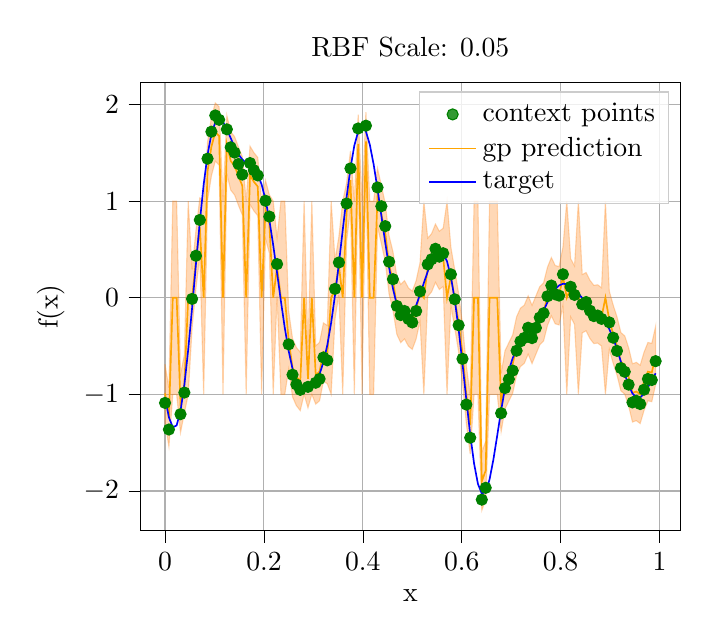
\begin{tikzpicture}

\definecolor{darkgray176}{RGB}{176,176,176}
\definecolor{darkorange25512714}{RGB}{255,127,14}
\definecolor{green}{RGB}{0,128,0}
\definecolor{lightgray204}{RGB}{204,204,204}
\definecolor{orange}{RGB}{255,165,0}

\begin{axis}[
legend cell align={left},
legend style={fill opacity=0.8, draw opacity=1, text opacity=1, draw=lightgray204},
tick align=outside,
tick pos=left,
title={RBF Scale: 0.05},
x grid style={darkgray176},
xlabel={x},
xmajorgrids,
xmin=-0.049609375, xmax=1.041796875,
xtick style={color=black},
y grid style={darkgray176},
ylabel={f(x)},
ymajorgrids,
ymin=-2.41224553995949, ymax=2.22731967114439,
ytick style={color=black}
]
\path [draw=darkorange25512714, fill=darkorange25512714, opacity=0.3]
(axis cs:0,-0.688383328985389)
--(axis cs:0,-1.29140601814092)
--(axis cs:0.0078125,-1.5413831705177)
--(axis cs:0.015625,-1)
--(axis cs:0.0234375,-1)
--(axis cs:0.03125,-1.39722157817871)
--(axis cs:0.0390625,-1.19397662668188)
--(axis cs:0.046875,-1)
--(axis cs:0.0546875,-0.312615969509551)
--(axis cs:0.0625,0.0932374694935545)
--(axis cs:0.0703125,0.430423814398134)
--(axis cs:0.078125,-1)
--(axis cs:0.0859375,1.00660140596913)
--(axis cs:0.09375,1.26045424831494)
--(axis cs:0.1015625,1.41340765421142)
--(axis cs:0.109375,1.37199936832405)
--(axis cs:0.1171875,-1)
--(axis cs:0.125,1.28255494331056)
--(axis cs:0.1328125,1.11365753849997)
--(axis cs:0.140625,1.06352678776651)
--(axis cs:0.1484375,0.956532171873315)
--(axis cs:0.15625,0.856964259341907)
--(axis cs:0.1640625,-1)
--(axis cs:0.171875,0.965423036921057)
--(axis cs:0.1796875,0.89815274910732)
--(axis cs:0.1875,0.8489957996014)
--(axis cs:0.1953125,-1)
--(axis cs:0.203125,0.610918073287938)
--(axis cs:0.2109375,0.461912394270764)
--(axis cs:0.21875,-1)
--(axis cs:0.2265625,0.0152650413264633)
--(axis cs:0.234375,-1)
--(axis cs:0.2421875,-1)
--(axis cs:0.25,-0.740297259312786)
--(axis cs:0.2578125,-1.02614532124722)
--(axis cs:0.265625,-1.11755500873782)
--(axis cs:0.2734375,-1.16809834347397)
--(axis cs:0.28125,-1)
--(axis cs:0.2890625,-1.13998389361326)
--(axis cs:0.296875,-1)
--(axis cs:0.3046875,-1.10139643136165)
--(axis cs:0.3125,-1.06571634374099)
--(axis cs:0.3203125,-0.863651326395437)
--(axis cs:0.328125,-0.890382622091687)
--(axis cs:0.3359375,-1)
--(axis cs:0.34375,-0.218288157083889)
--(axis cs:0.3515625,0.0299163128477336)
--(axis cs:0.359375,-1)
--(axis cs:0.3671875,0.584659180134388)
--(axis cs:0.375,0.915193592947601)
--(axis cs:0.3828125,-1)
--(axis cs:0.390625,1.290893798502)
--(axis cs:0.3984375,-1)
--(axis cs:0.40625,1.31714457989889)
--(axis cs:0.4140625,-1)
--(axis cs:0.421875,-1)
--(axis cs:0.4296875,0.735886932895363)
--(axis cs:0.4375,0.559125384839859)
--(axis cs:0.4453125,0.371735822723044)
--(axis cs:0.453125,0.0368862627547937)
--(axis cs:0.4609375,-0.127295112219921)
--(axis cs:0.46875,-0.378900165420577)
--(axis cs:0.4765625,-0.464845701930011)
--(axis cs:0.484375,-0.426493428332804)
--(axis cs:0.4921875,-0.50154131099667)
--(axis cs:0.5,-0.534409846037235)
--(axis cs:0.5078125,-0.426543569491712)
--(axis cs:0.515625,-0.241967819964512)
--(axis cs:0.5234375,-1)
--(axis cs:0.53125,0.0122248665430005)
--(axis cs:0.5390625,0.0602919132122145)
--(axis cs:0.546875,0.158896214718978)
--(axis cs:0.5546875,0.0846877741175106)
--(axis cs:0.5625,0.116868292496573)
--(axis cs:0.5703125,-1)
--(axis cs:0.578125,-0.0813338984325448)
--(axis cs:0.5859375,-0.316384265851202)
--(axis cs:0.59375,-0.560231258330496)
--(axis cs:0.6015625,-0.876462848827993)
--(axis cs:0.609375,-1.30663025659162)
--(axis cs:0.6171875,-1.61851670489081)
--(axis cs:0.625,-1)
--(axis cs:0.6328125,-1)
--(axis cs:0.640625,-2.20135621218204)
--(axis cs:0.6484375,-2.08992262848657)
--(axis cs:0.65625,-1)
--(axis cs:0.6640625,-1)
--(axis cs:0.671875,-1)
--(axis cs:0.6796875,-1.38823123426756)
--(axis cs:0.6875,-1.15162244906953)
--(axis cs:0.6953125,-1.06873940030507)
--(axis cs:0.703125,-0.987399313245003)
--(axis cs:0.7109375,-0.800413053019892)
--(axis cs:0.71875,-0.711758029811619)
--(axis cs:0.7265625,-0.679632507817893)
--(axis cs:0.734375,-0.583887351931207)
--(axis cs:0.7421875,-0.681631199463245)
--(axis cs:0.75,-0.584985494806654)
--(axis cs:0.7578125,-0.488159440646371)
--(axis cs:0.765625,-0.447267140033861)
--(axis cs:0.7734375,-0.287496374950949)
--(axis cs:0.78125,-0.186992655461015)
--(axis cs:0.7890625,-0.269502708169921)
--(axis cs:0.796875,-0.281603215293504)
--(axis cs:0.8046875,-0.0812010894034952)
--(axis cs:0.8125,-1)
--(axis cs:0.8203125,-0.198774182942497)
--(axis cs:0.828125,-0.275112009113055)
--(axis cs:0.8359375,-1)
--(axis cs:0.84375,-0.363647653058834)
--(axis cs:0.8515625,-0.34228646896296)
--(axis cs:0.859375,-0.423369229554881)
--(axis cs:0.8671875,-0.474572072217907)
--(axis cs:0.875,-0.469278532642914)
--(axis cs:0.8828125,-0.500621643663753)
--(axis cs:0.890625,-1)
--(axis cs:0.8984375,-0.53333254879791)
--(axis cs:0.90625,-0.677590134405544)
--(axis cs:0.9140625,-0.801608029662508)
--(axis cs:0.921875,-0.963462625849322)
--(axis cs:0.9296875,-0.998288812851843)
--(axis cs:0.9375,-1.1192513280054)
--(axis cs:0.9453125,-1.2865681735166)
--(axis cs:0.953125,-1.27205635452423)
--(axis cs:0.9609375,-1.3019123402926)
--(axis cs:0.96875,-1.16662625583365)
--(axis cs:0.9765625,-1.06622264929502)
--(axis cs:0.984375,-1.07593145893693)
--(axis cs:0.9921875,-0.898316631155426)
--(axis cs:0.9921875,-0.295293941999899)
--(axis cs:0.9921875,-0.295293941999899)
--(axis cs:0.984375,-0.472908769781403)
--(axis cs:0.9765625,-0.463199960139497)
--(axis cs:0.96875,-0.563603566678123)
--(axis cs:0.9609375,-0.698889651137071)
--(axis cs:0.953125,-0.669033665368699)
--(axis cs:0.9453125,-0.683545484361075)
--(axis cs:0.9375,-0.516228638849877)
--(axis cs:0.9296875,-0.395266123696316)
--(axis cs:0.921875,-0.360439936693794)
--(axis cs:0.9140625,-0.19858534050698)
--(axis cs:0.90625,-0.0745674452500167)
--(axis cs:0.8984375,0.0696901403576179)
--(axis cs:0.890625,1)
--(axis cs:0.8828125,0.102401045491775)
--(axis cs:0.875,0.133744156512613)
--(axis cs:0.8671875,0.12845061693762)
--(axis cs:0.859375,0.179653459600647)
--(axis cs:0.8515625,0.260736220192568)
--(axis cs:0.84375,0.239375036096694)
--(axis cs:0.8359375,1)
--(axis cs:0.828125,0.327910680042473)
--(axis cs:0.8203125,0.404248506213031)
--(axis cs:0.8125,1)
--(axis cs:0.8046875,0.521821599752032)
--(axis cs:0.796875,0.321419473862024)
--(axis cs:0.7890625,0.333519980985607)
--(axis cs:0.78125,0.416030033694513)
--(axis cs:0.7734375,0.315526314204578)
--(axis cs:0.765625,0.155755549121667)
--(axis cs:0.7578125,0.114863248509157)
--(axis cs:0.75,0.0180371943488732)
--(axis cs:0.7421875,-0.0786085103077172)
--(axis cs:0.734375,0.0191353372243203)
--(axis cs:0.7265625,-0.0766098186623656)
--(axis cs:0.71875,-0.108735340656092)
--(axis cs:0.7109375,-0.197390363864365)
--(axis cs:0.703125,-0.384376624089476)
--(axis cs:0.6953125,-0.465716711149538)
--(axis cs:0.6875,-0.548599759914007)
--(axis cs:0.6796875,-0.785208545112036)
--(axis cs:0.671875,1)
--(axis cs:0.6640625,1)
--(axis cs:0.65625,1)
--(axis cs:0.6484375,-1.48689993933105)
--(axis cs:0.640625,-1.59833352302651)
--(axis cs:0.6328125,1)
--(axis cs:0.625,1)
--(axis cs:0.6171875,-1.01549401573528)
--(axis cs:0.609375,-0.70360756743609)
--(axis cs:0.6015625,-0.273440159672465)
--(axis cs:0.59375,0.0427914308250313)
--(axis cs:0.5859375,0.286638423304326)
--(axis cs:0.578125,0.521688790722983)
--(axis cs:0.5703125,1)
--(axis cs:0.5625,0.719890981652101)
--(axis cs:0.5546875,0.687710463273038)
--(axis cs:0.546875,0.761918903874506)
--(axis cs:0.5390625,0.663314602367742)
--(axis cs:0.53125,0.615247555698528)
--(axis cs:0.5234375,1)
--(axis cs:0.515625,0.361054869191016)
--(axis cs:0.5078125,0.176479119663816)
--(axis cs:0.5,0.0686128431182931)
--(axis cs:0.4921875,0.101481378158857)
--(axis cs:0.484375,0.176529260822724)
--(axis cs:0.4765625,0.138176987225517)
--(axis cs:0.46875,0.224122523734951)
--(axis cs:0.4609375,0.475727576935606)
--(axis cs:0.453125,0.639908951910321)
--(axis cs:0.4453125,0.974758511878572)
--(axis cs:0.4375,1.16214807399539)
--(axis cs:0.4296875,1.33890962205089)
--(axis cs:0.421875,1)
--(axis cs:0.4140625,1)
--(axis cs:0.40625,1.92016726905442)
--(axis cs:0.3984375,1)
--(axis cs:0.390625,1.89391648765753)
--(axis cs:0.3828125,1)
--(axis cs:0.375,1.51821628210313)
--(axis cs:0.3671875,1.18768186928992)
--(axis cs:0.359375,1)
--(axis cs:0.3515625,0.632939002003261)
--(axis cs:0.34375,0.384734532071639)
--(axis cs:0.3359375,1)
--(axis cs:0.328125,-0.287359932936159)
--(axis cs:0.3203125,-0.260628637239909)
--(axis cs:0.3125,-0.462693654585458)
--(axis cs:0.3046875,-0.498373742206126)
--(axis cs:0.296875,1)
--(axis cs:0.2890625,-0.536961204457736)
--(axis cs:0.28125,1)
--(axis cs:0.2734375,-0.565075654318443)
--(axis cs:0.265625,-0.514532319582289)
--(axis cs:0.2578125,-0.423122632091688)
--(axis cs:0.25,-0.137274570157258)
--(axis cs:0.2421875,1)
--(axis cs:0.234375,1)
--(axis cs:0.2265625,0.618287730481991)
--(axis cs:0.21875,1)
--(axis cs:0.2109375,1.06493508342629)
--(axis cs:0.203125,1.21394076244347)
--(axis cs:0.1953125,1)
--(axis cs:0.1875,1.45201848875693)
--(axis cs:0.1796875,1.50117543826285)
--(axis cs:0.171875,1.56844572607658)
--(axis cs:0.1640625,1)
--(axis cs:0.15625,1.45998694849743)
--(axis cs:0.1484375,1.55955486102884)
--(axis cs:0.140625,1.66654947692204)
--(axis cs:0.1328125,1.7166802276555)
--(axis cs:0.125,1.88557763246609)
--(axis cs:0.1171875,1)
--(axis cs:0.109375,1.97502205747958)
--(axis cs:0.1015625,2.01643034336694)
--(axis cs:0.09375,1.86347693747047)
--(axis cs:0.0859375,1.60962409512466)
--(axis cs:0.078125,1)
--(axis cs:0.0703125,1.03344650355366)
--(axis cs:0.0625,0.696260158649082)
--(axis cs:0.0546875,0.290406719645977)
--(axis cs:0.046875,1)
--(axis cs:0.0390625,-0.590953937526351)
--(axis cs:0.03125,-0.794198889023184)
--(axis cs:0.0234375,1)
--(axis cs:0.015625,1)
--(axis cs:0.0078125,-0.938360481362176)
--(axis cs:0,-0.688383328985389)
--cycle;

\addplot [draw=green, fill=green, mark=*, only marks]
table{%
x  y
0 -1.08888411521912
0.0078125 -1.36385905742645
0.03125 -1.20528125762939
0.0390625 -0.981711804866791
0.0546875 -0.0122150871902704
0.0625 0.434223681688309
0.0703125 0.805128693580627
0.0859375 1.43892407417297
0.09375 1.71816217899323
0.1015625 1.88641095161438
0.109375 1.84086179733276
0.125 1.74247288703918
0.1328125 1.55668580532074
0.140625 1.50154197216034
0.1484375 1.38384783267975
0.15625 1.27432310581207
0.171875 1.39362776279449
0.1796875 1.31963050365448
0.1875 1.26555788516998
0.203125 1.0036723613739
0.2109375 0.839766085147858
0.2265625 0.348454028367996
0.25 -0.482664495706558
0.2578125 -0.797097384929657
0.265625 -0.89764803647995
0.2734375 -0.95324569940567
0.2890625 -0.922319829463959
0.3046875 -0.87987357378006
0.3125 -0.840625524520874
0.3203125 -0.618353962898254
0.328125 -0.647758424282074
0.34375 0.091545507311821
0.3515625 0.364570409059525
0.3671875 0.974787592887878
0.375 1.3383754491806
0.390625 1.75164568424225
0.40625 1.78052151203156
0.4296875 1.14113807678223
0.4375 0.946700394153595
0.4453125 0.740571856498718
0.453125 0.372237354516983
0.4609375 0.191637858748436
0.46875 -0.0851277038455009
0.4765625 -0.179667785763741
0.484375 -0.137480288743973
0.4921875 -0.220032960176468
0.5 -0.256188362836838
0.5078125 -0.137535452842712
0.515625 0.065497875213623
0.53125 0.345109820365906
0.5390625 0.397983580827713
0.546875 0.506448328495026
0.5546875 0.424819022417068
0.5625 0.460217595100403
0.578125 0.242195188999176
0.5859375 -0.0163602139800787
0.59375 -0.284591913223267
0.6015625 -0.632446646690369
0.609375 -1.1056307554245
0.6171875 -1.44870591163635
0.640625 -2.08982944488525
0.6484375 -1.96725237369537
0.6796875 -1.19539189338684
0.6875 -0.935122191905975
0.6953125 -0.843950867652893
0.703125 -0.75447678565979
0.7109375 -0.548791885375977
0.71875 -0.45127135515213
0.7265625 -0.415933281183243
0.734375 -0.310613602399826
0.7421875 -0.418131828308105
0.75 -0.311821579933167
0.7578125 -0.20531290769577
0.765625 -0.16033136844635
0.7734375 0.0154164666309953
0.78125 0.125970557332039
0.7890625 0.0352094992995262
0.796875 0.0218989420682192
0.8046875 0.242341279983521
0.8203125 0.113010875880718
0.828125 0.0290392693132162
0.84375 -0.0683499425649643
0.8515625 -0.0448526367545128
0.859375 -0.134043678641319
0.8671875 -0.190366804599762
0.875 -0.184543907642365
0.8828125 -0.219021335244179
0.8984375 -0.255003333091736
0.90625 -0.413686662912369
0.9140625 -0.550106346607208
0.921875 -0.728146433830261
0.9296875 -0.766455233097076
0.9375 -0.899513959884644
0.9453125 -1.08356249332428
0.953125 -1.0675995349884
0.9609375 -1.1004410982132
0.96875 -0.951626420021057
0.9765625 -0.84118241071701
0.984375 -0.851862132549286
0.9921875 -0.656485795974731
};
\addlegendentry{context points}
\addplot [semithick, orange]
table {%
0 -0.989894673563153
0.0078125 -1.23987182593994
0.015625 -8.63182962435564e-81
0.0234375 -7.62819499260482e-81
0.03125 -1.09571023360095
0.0390625 -0.892465282104115
0.046875 -6.29053852829941e-81
0.0546875 -0.0111046249317873
0.0625 0.394748814071318
0.0703125 0.731935158975898
0.078125 1.42025535318319e-80
0.0859375 1.30811275054689
0.09375 1.56196559289271
0.1015625 1.71491899878918
0.109375 1.67351071290182
0.1171875 2.26788358850887e-80
0.125 1.58406628788832
0.1328125 1.41516888307773
0.140625 1.36503813234428
0.1484375 1.25804351645108
0.15625 1.15847560391967
0.1640625 1.68853951879024e-80
0.171875 1.26693438149882
0.1796875 1.19966409368508
0.1875 1.15050714417916
0.1953125 1.43619014134169e-80
0.203125 0.912429417865702
0.2109375 0.763423738848528
0.21875 7.5202155916508e-81
0.2265625 0.316776385904227
0.234375 2.20535682393606e-81
0.2421875 -3.05477161294021e-81
0.25 -0.438785914735022
0.2578125 -0.724633976669452
0.265625 -0.816043664160053
0.2734375 -0.866586998896207
0.28125 -1.18704072543765e-80
0.2890625 -0.8384725490355
0.296875 -1.14060370437407e-80
0.3046875 -0.79988508678389
0.3125 -0.764204999163222
0.3203125 -0.562139981817673
0.328125 -0.588871277513923
0.3359375 -3.52025755535937e-81
0.34375 0.0832231874938751
0.3515625 0.331427657425497
0.359375 8.47676335509911e-81
0.3671875 0.886170524712152
0.375 1.21670493752536
0.3828125 1.95566663460928e-80
0.390625 1.59240514307976
0.3984375 2.23549978866154e-80
0.40625 1.61865592447665
0.4140625 1.12688762404417e-80
0.421875 7.22223458620296e-81
0.4296875 1.03739827747313
0.4375 0.860636729417622
0.4453125 0.673247167300808
0.453125 0.338397607332558
0.4609375 0.174216232357843
0.46875 -0.0773888208428133
0.4765625 -0.163334357352247
0.484375 -0.12498208375504
0.4921875 -0.200029966418907
0.5 -0.232898501459471
0.5078125 -0.125032224913948
0.515625 0.0595435246132523
0.5234375 2.59872594381364e-81
0.53125 0.313736211120764
0.5390625 0.361803257789978
0.546875 0.460407559296742
0.5546875 0.386199118695274
0.5625 0.418379637074337
0.5703125 4.44555302608877e-81
0.578125 0.220177446145219
0.5859375 -0.0148729212734377
0.59375 -0.258719913752733
0.6015625 -0.574951504250229
0.609375 -1.00511891201385
0.6171875 -1.31700536031305
0.625 -9.1688234596225e-81
0.6328125 -1.32264778235929e-80
0.640625 -1.89984486760428
0.6484375 -1.78841128390881
0.65625 -1.24506914166145e-80
0.6640625 -6.74399606573302e-321
0.671875 -7.56560536413778e-81
0.6796875 -1.0867198896898
0.6875 -0.850111104491771
0.6953125 -0.767228055727302
0.703125 -0.68588796866724
0.7109375 -0.498901708442128
0.71875 -0.410246685233856
0.7265625 -0.378121163240129
0.734375 -0.282376007353444
0.7421875 -0.380119854885481
0.75 -0.283474150228891
0.7578125 -0.186648096068607
0.765625 -0.145755795456097
0.7734375 0.0140149696268144
0.78125 0.114518689116749
0.7890625 0.0320086364078432
0.796875 0.0199081292842603
0.8046875 0.220310255174269
0.8125 2.2490149418296e-81
0.8203125 0.102737161635267
0.828125 0.0263993354647092
0.8359375 -2.48796251285932e-82
0.84375 -0.0621363084810699
0.8515625 -0.0407751243851963
0.859375 -0.121857884977117
0.8671875 -0.173060727640144
0.875 -0.16776718806515
0.8828125 -0.199110299085989
0.890625 -3.00009020165606e-81
0.8984375 -0.231821204220146
0.90625 -0.376078789827781
0.9140625 -0.500096685084744
0.921875 -0.661951281271558
0.9296875 -0.69677746827408
0.9375 -0.817739983427641
0.9453125 -0.985056828938838
0.953125 -0.970545009946463
0.9609375 -1.00040099571483
0.96875 -0.865114911255886
0.9765625 -0.764711304717261
0.984375 -0.774420114359166
0.9921875 -0.596805286577663
};
\addlegendentry{gp prediction}
\addplot [semithick, blue]
table {%
0 -1.03190088272095
0.0078125 -1.23832082748413
0.015625 -1.34114527702332
0.0234375 -1.32112503051758
0.03125 -1.17219460010529
0.0390625 -0.903067886829376
0.046875 -0.536460399627686
0.0546875 -0.106029771268368
0.0625 0.348389685153961
0.0703125 0.786377489566803
0.078125 1.17235600948334
0.0859375 1.47996890544891
0.09375 1.69477891921997
0.1015625 1.81499648094177
0.109375 1.85029745101929
0.1171875 1.81907176971436
0.125 1.74464392662048
0.1328125 1.65108573436737
0.140625 1.5592485666275
0.1484375 1.48356473445892
0.15625 1.43004608154297
0.1640625 1.39574778079987
0.171875 1.36977696418762
0.1796875 1.33572459220886
0.1875 1.27517974376678
0.1953125 1.17177939414978
0.203125 1.01506853103638
0.2109375 0.803369522094727
0.21875 0.544939458370209
0.2265625 0.256988525390625
0.234375 -0.0373827256262302
0.2421875 -0.31369349360466
0.25 -0.550928950309753
0.2578125 -0.735419094562531
0.265625 -0.862659752368927
0.2734375 -0.936571002006531
0.28125 -0.966469764709473
0.2890625 -0.962743639945984
0.296875 -0.932617247104645
0.3046875 -0.877354919910431
0.3125 -0.79178786277771
0.3203125 -0.666325271129608
0.328125 -0.490849494934082
0.3359375 -0.259326338768005
0.34375 0.0262537952512503
0.3515625 0.353797823190689
0.359375 0.701548218727112
0.3671875 1.04097235202789
0.375 1.34135222434998
0.3828125 1.57489681243896
0.390625 1.72113740444183
0.3984375 1.76968026161194
0.40625 1.72093117237091
0.4140625 1.5849871635437
0.421875 1.37929701805115
0.4296875 1.12583386898041
0.4375 0.848393142223358
0.4453125 0.570347785949707
0.453125 0.312901496887207
0.4609375 0.0937184765934944
0.46875 -0.0741947144269943
0.4765625 -0.183340907096863
0.484375 -0.232152581214905
0.4921875 -0.224762991070747
0.5 -0.170023009181023
0.5078125 -0.0799106359481812
0.515625 0.0322536490857601
0.5234375 0.153246462345123
0.53125 0.270607441663742
0.5390625 0.372446179389954
0.546875 0.446724712848663
0.5546875 0.480664193630219
0.5625 0.460967868566513
0.5703125 0.375286787748337
0.578125 0.214874431490898
0.5859375 -0.0221472587436438
0.59375 -0.327864438295364
0.6015625 -0.683051466941833
0.609375 -1.057896733284
0.6171875 -1.41531252861023
0.625 -1.71648979187012
0.6328125 -1.92767524719238
0.640625 -2.0266592502594
0.6484375 -2.00734686851501
0.65625 -1.88113224506378
0.6640625 -1.67455267906189
0.671875 -1.42367446422577
0.6796875 -1.16656041145325
0.6875 -0.935693144798279
0.6953125 -0.752215683460236
0.703125 -0.623294651508331
0.7109375 -0.542998433113098
0.71875 -0.496118426322937
0.7265625 -0.463622778654099
0.734375 -0.428145885467529
0.7421875 -0.378092586994171
0.75 -0.309508740901947
0.7578125 -0.22560116648674
0.765625 -0.13447293639183
0.7734375 -0.0460650362074375
0.78125 0.0306433904916048
0.7890625 0.089411273598671
0.796875 0.127238944172859
0.8046875 0.143865555524826
0.8125 0.140849381685257
0.8203125 0.120811343193054
0.828125 0.0871279388666153
0.8359375 0.0439450740814209
0.84375 -0.0039005228318274
0.8515625 -0.0514686331152916
0.859375 -0.0949170738458633
0.8671875 -0.132983282208443
0.875 -0.168070718646049
0.8828125 -0.206248894333839
0.890625 -0.255822032690048
0.8984375 -0.324701368808746
0.90625 -0.417362183332443
0.9140625 -0.532440483570099
0.921875 -0.661884367465973
0.9296875 -0.792080819606781
0.9375 -0.906728088855743
0.9453125 -0.99066162109375
0.953125 -1.03355658054352
0.9609375 -1.03250002861023
0.96875 -0.992771685123444
0.9765625 -0.926686108112335
0.984375 -0.850848078727722
0.9921875 -0.782549917697906
};
\addlegendentry{target}
\end{axis}

\end{tikzpicture}

	}
	\caption{Gaussian Process function estimation on four example data frames with varying number of context points. Functions have been sampled from a multivariate normal distribution with an RBF kernel.}
	\label{fig:gaussian}
\end{figure*}

For real-world scenarios, we cannot assume to know the prior distribution beforehand. Rather, we want to work with unseen functions directly without any prior knowledge, which inevitably introduces bias. We need to have a model that estimates the underlying function given only some context points and can impute missing values based on that. This in-context zero-shot function estimation can be split up into two subtasks. First, process the context points so that we get a representation of the underlying function and then predict the value of that function at a certain point.

\citet{Lu_2021} train two neural networks for their DeepONet, that tackles these subtasks. The Branch net learns an operator $G: u\rightarrow G(u)$ with $u$ being the sequence of context points and the result $G(u)$ is supposed to represent the underlying function. Using this representation and given an arbitrary point $y$, the Trunk net predicts the value $G(u)(y)$. \cite{Lu_2021}

Neural networks are not well fit to handle sequences of varying length, as we expect with the sequence of context points having a different length depending on the specific use case. \citet{seifner2025zeroshotimputationfoundationinference} use a bi-directional LSTM that acts like the Branch net from DeepONets and allows processing sequences of varying length. Adapting their approach, we use a transformer to model sequences of varying length.